\documentclass{article}
\usepackage{graphicx} % Extended graphics inclusions
\usepackage{float}
\usepackage{url} % For \url{}
\usepackage{../config/atxy} % For front cover
\usepackage{amsfonts} % Needed for some fonts
\usepackage[usenames]{color} % Needed for colored R input/output
\usepackage{pdfcolmk} % Correct some problems with the color stack


\title{RISA \textit{in silico} with seqinR}
\author{Lobry, J.R.}

\usepackage{/Library/Frameworks/R.framework/Resources/share/texmf/Sweave}
\begin{document}
%
% To change the R input/output style:
%
\definecolor{Soutput}{rgb}{0,0,0.56}
\definecolor{Sinput}{rgb}{0.56,0,0}
\DefineVerbatimEnvironment{Sinput}{Verbatim}
{formatcom={\color{Sinput}},fontsize=\footnotesize, baselinestretch=0.75}
\DefineVerbatimEnvironment{Soutput}{Verbatim}
{formatcom={\color{Soutput}},fontsize=\footnotesize, baselinestretch=0.75}
%
% This removes the extra spacing after code and output chunks in Sweave,
% but keeps the spacing around the whole block.
%
\fvset{listparameters={\setlength{\topsep}{0pt}}}
\renewenvironment{Schunk}{\vspace{\topsep}}{\vspace{\topsep}}
%
% Rlogo
%
\newcommand{\Rlogo}{\protect
\includegraphics[height=1.8ex,keepaspectratio]{../figs/Rlogo.pdf}}
%
% Shortcut for seqinR:
%
\newcommand{\seqinr}{\texttt{seqin\bf{R}}}
\newcommand{\Seqinr}{\texttt{Seqin\bf{R}}}
\fvset{fontsize= \scriptsize}
%
% R output options and libraries to be loaded.
%
%
%  Sweave Options
%
% Put all figures in the fig folder and start the name with current file name.
% Do not produce EPS files
%


\maketitle
\tableofcontents
% BEGIN - DO NOT REMOVE THIS LINE

\section{Introduction}

By RISA we mean here Ribosomal Intergenic Spacer Analysis. Ribosomal
genes are highly conserved so that it is relatively easy to design
universal PCR primers. On the other hand the intergenic space is under
weaker selective pressure, yielding more between species variability
in terms of length.

Making a RISA \textit{in silico} is an interesting task for seqinR :
we want to extract ribosomal genes from general databases and then
to compute the fragment length between the two primers.

\section{The primers}

Let's use the following primer in the 16S, also known as 
S-D-Bact-1522-b-S-20 \cite{RanjardL2000}:

\begin{Schunk}
\begin{Sinput}
 library(seqinr)
 (amo1 <- tolower("TGCGGCTGGATCCCCTCCTT"))
\end{Sinput}
\begin{Soutput}
[1] "tgcggctggatcccctcctt"
\end{Soutput}
\end{Schunk}


Let's use the following primer in the 23S, also known as 
L-D-Bact-132-a-A-18 \cite{RanjardL2000}:

\begin{Schunk}
\begin{Sinput}
 (amo2 <- tolower("CCGGGTTTCCCCATTCGG"))
\end{Sinput}
\begin{Soutput}
[1] "ccgggtttccccattcgg"
\end{Soutput}
\end{Schunk}

We work thereafter with its complementary sequence as follows:

\begin{Schunk}
\begin{Sinput}
 cplt <- function(x) c2s(comp(rev(s2c(x))))
 (amo2 <- cplt(amo2))
\end{Sinput}
\begin{Soutput}
[1] "ccgaatggggaaacccgg"
\end{Soutput}
\end{Schunk}

\section{Finding a primer location}

We want to fing a substring allowing for mismatches (say 3). Let's
write a function for this. Here we just use a moving window to count the
number of matches for all positions and return the one with the
maximum value. If the maximum number of matches if not enough, \texttt{NA}
is returned instead.

\begin{Schunk}
\begin{Sinput}
 find.amo <- function(amo, myseq, verbose = FALSE, nmiss = 3) {
     y <- numeric(nchar(myseq))
     myseq2 <- s2c(myseq)
     for (k in seq_len(nchar(myseq) - nchar(amo))) {
         y[k] <- sum(s2c(amo) == myseq2[k:(k + nchar(amo) - 
             1)])
     }
     if (verbose) 
         plot(1:nchar(myseq), y, type = "h", ylim = c(0, nchar(amo)), 
             main = amo)
     nmismatch <- nchar(amo) - max(y)
     if (verbose) 
         print(paste(nmismatch, "mismatch"))
     if (nmismatch > nmiss) {
         warning(paste("too many mismatches:", nmismatch))
         return(NA)
     }
     if (verbose) 
         rug(which.max(y), col = "red")
     return(which.max(y))
 }
\end{Sinput}
\end{Schunk}

Example with a random sequence:

\begin{Schunk}
\begin{Sinput}
 rseq <- c2s(sample(s2c("acgt"), 1000, rep = T))
 find.amo(amo1, rseq, verb = T)
\end{Sinput}
\begin{Soutput}
[1] "8 mismatch"
[1] NA
\end{Soutput}
\end{Schunk}
\includegraphics{../figs/risa-essai}

Now insert a perfect target :

\begin{Schunk}
\begin{Sinput}
 substr(rseq, 100, 100 + nchar(amo1)) <- amo1
 find.amo(amo1, rseq, verb = T)
\end{Sinput}
\begin{Soutput}
[1] "0 mismatch"
[1] 100
\end{Soutput}
\end{Schunk}
\includegraphics{../figs/risa-essai2}

\section{Compute the length of the intergenic space}

More exactly we want to compute the length of the fragment amplified
between two PCR primers. Here it is, note that we have to take into account
whether the primers are on the direct or complementary strand and the
length of the primers:

\begin{Schunk}
\begin{Sinput}
 risa.length <- function(myseq, amo1, amo2, forward, verbose = FALSE) {
     if (forward) {
         posamo1 <- find.amo(amo1, myseq, verbose = verbose)
         posamo2 <- find.amo(amo2, myseq, verbose = verbose)
     }
     else {
         posamo1 <- find.amo(cplt(amo1), myseq, verbose = verbose)
         posamo2 <- find.amo(cplt(amo2), myseq, verbose = verbose)
     }
     if (is.na(posamo1)) 
         return(list(res = NA, posamo1 = NA, posamo2 = NA))
     if (is.na(posamo2)) 
         return(list(res = NA, posamo1 = NA, posamo2 = NA))
     return(list(res = abs(posamo2 - posamo1) + ifelse(forward, 
         nchar(amo2), nchar(amo1)), posamo1 = posamo1, posamo2 = posamo2))
 }
\end{Sinput}
\end{Schunk}

Let's check this with an artificial example by inserting the second primer at
position 300 in our random sequence:

\begin{Schunk}
\begin{Sinput}
 nchar(amo2)
\end{Sinput}
\begin{Soutput}
[1] 18
\end{Soutput}
\begin{Sinput}
 substr(rseq, 300, 300 + nchar(amo2)) <- amo2
 risa.length(rseq, amo1, amo2, forward = T)$res
\end{Sinput}
\begin{Soutput}
[1] 218
\end{Soutput}
\begin{Sinput}
 risa.length(cplt(rseq), amo1, amo2, forward = F)$res
\end{Sinput}
\begin{Soutput}
[1] 218
\end{Soutput}
\end{Schunk}

Looks OK for me.

\section{Compute IGS for a sequence fragment}

\begin{figure}
\centering
\fbox{
\begin{minipage}{\textwidth}
\centering
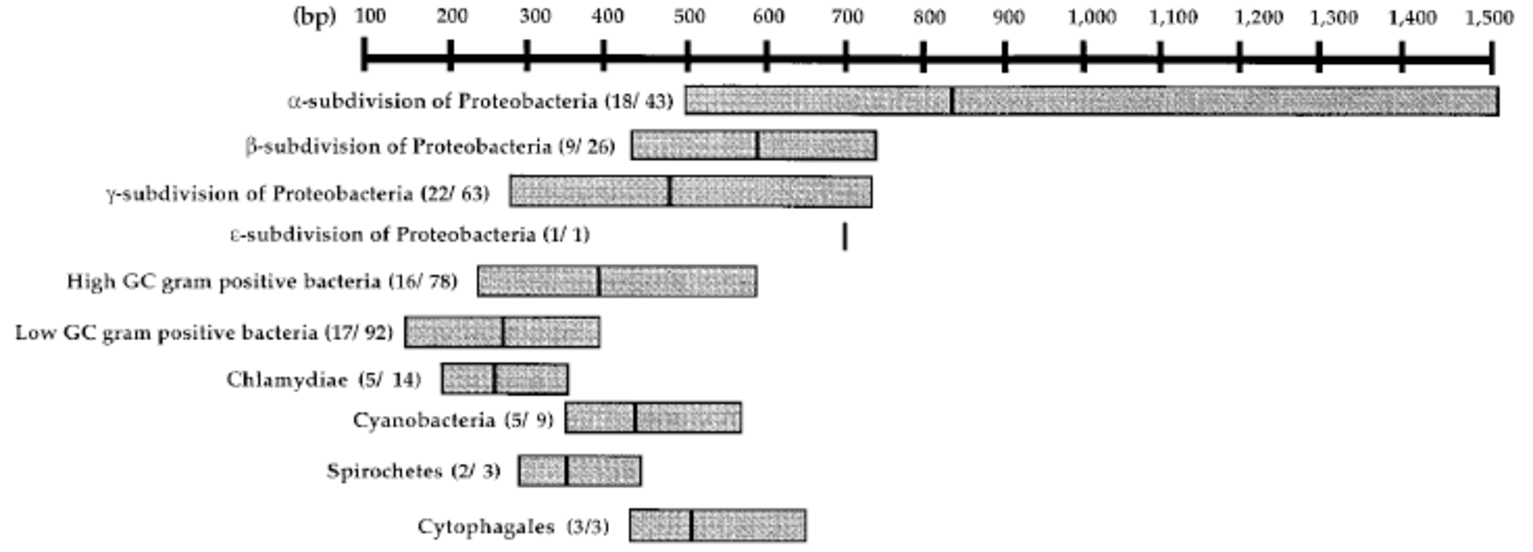
\includegraphics[width=\textwidth]{../figs/fig1RanjardL2000}
\caption{Screenshort of a part of figure 1 in \cite{RanjardL2000} showing the observed range
of ribosomal intergenic space length in bacterial species (n = 428).}
\label{fig1RanjardL2000}
\end{minipage}
}
\end{figure}


By sequence fragment we mean here a genbank entry accessed
by its name (\texttt{mnemo} in the code thereafter).
There could be more than one rRNA operon in the sequence fragment
but there should be the same number of 16S and 23S genes.
There is a maximum length to avoid problems when genes are
not annotated in consecutive order, in this case \texttt{NA}
is returned. The default maximum length of 10 kb is conservative,
the maximum observed value is 1.5 kb (\textit{cf} Fig. \ref{fig1RanjardL2000}),
some post-processing of the results is most likely necessary to remove outliers.

\begin{Schunk}
\begin{Sinput}
 mn2risa <- function(mnemo, amo1, amo2, maxlength = 10000, 
     verbose = FALSE) {
     if (verbose) 
         print(paste("mn2risa -->", mnemo))
     query("frag", paste("N=", mnemo))
     query("frag16S", "frag ET T=RRNA ET K=16S@")
     if (verbose) 
         print(paste("n 16S = ", frag16S$nelem))
     query("frag23S", "frag ET T=RRNA ET K=23S@")
     if (verbose) 
         print(paste("n 23S = ", frag23S$nelem))
     if (frag16S$nelem != frag23S$nelem) 
         return(NA)
     n <- frag16S$nelem
     loc1 <- getLocation(frag16S)
     loc2 <- getLocation(frag23S)
     risa <- numeric(n)
     for (i in seq_len(n)) {
         coords <- c(loc1[[i]], loc2[[i]])
         if (coords[1] < coords[3]) {
             forward <- TRUE
             if (verbose) 
                 print("forward")
         }
         else {
             forward <- FALSE
             if (verbose) 
                 print("bacward")
         }
         if (verbose) 
             print(coords)
         xmin <- min(coords)
         xmax <- max(coords)
         if (xmax - xmin > maxlength) 
             return(NA)
         myseq <- as.character(getFrag(frag$req[[1]], xmin, 
             xmax))
         if (verbose) 
             print(paste("nchar myseq = ", nchar(myseq)))
         risa[i] <- risa.length(myseq, amo1, amo2, forward, 
             verbose = F)$res
     }
     return(risa)
 }
\end{Sinput}
\end{Schunk}

Example with a fragment with one 16S and two 23S genes,
\texttt{NA} is returned as expected :

\begin{Schunk}
\begin{Sinput}
 mn2risa("BBRNAOPR", amo1, amo2, verb = T)
\end{Sinput}
\end{Schunk}

Example with a fragment with seven 16S and seven 23S genes,
the seven RISA length are returned :

\begin{Schunk}
\begin{Sinput}
 mn2risa("AE005174", amo1, amo2, verb = T)
\end{Sinput}
\end{Schunk}

\section{Compute IGS for a species}

We could work in fact at any taxonomical level, but suppose here that
we are interested by the species level. All we have to do is to find
the list of fragment where there is at least one 16S and one 23S gene.
We use here all the power of ACNUC query language.

\begin{Schunk}
\begin{Sinput}
 sp2risa <- function(sp, amo1, amo2, verbose = TRUE) {
     if (verbose) 
         print(paste("sp2risa -->", sp))
     query("cursp", paste("sp=", sp), virtual = TRUE)
     query("res1", "cursp ET T=RRNA ET K=16S@", virtual = TRUE)
     query("res1", "ME res1", virtual = TRUE)
     query("res2", "cursp ET T=RRNA ET K=23S@", virtual = TRUE)
     query("res2", "ME res2", virtual = TRUE)
     query("res3", "res1 ET res2")
     if (verbose) 
         print(paste("number of mother sequences = ", res3$nelem))
     seqnames <- getName(res3)
     result <- vector("list", res3$nelem)
     names(result) <- seqnames
     for (i in seq_len(res3$nelem)) {
         result[[i]] <- mn2risa(seqnames[i], amo1, amo2, verbose = verbose)
     }
     return(result)
 }
\end{Sinput}
\end{Schunk}


\section{Loop over many species}

We loop now over all bacterial species in genbank. As this is long, we run
it overnight in batch, saving results on the fly to spy them.
When the species name is a single word this is most likely a genus,
then to avoid redundancy in computation with the underlying species,
it is not considered and a \texttt{+Inf} value is set. An empty list
means that no fragment with both 16S and 23S genes were found. A
missing value \texttt{NA} means that the PCR primers were not found.

\begin{Schunk}
\begin{Sinput}
 query("all", "sp=bacteria", virtual = TRUE)
 query("allsp", "ps all")
 splist <- getName(allsp)
 resultat <- vector("list", length(splist))
 names(resultat) <- splist
 i <- 1
 for (sp in splist) {
     print(paste("===>", sp))
     if (length(unlist(strsplit(sp, split = " "))) == 1) {
         resultat[[i]] <- +Inf
         i <- i + 1
         next
     }
     resultat[[i]] <- sp2risa(sp = sp, amo1, amo2, verbose = TRUE)
     save(resultat, file = "resultat.RData")
     print(paste("=>", resultat[[i]]))
     i <- i + 1
 }
\end{Sinput}
\end{Schunk}

\section{Playing with results}



\section*{Session Informations}

This part was compiled under the following \Rlogo{}~environment:

\begin{itemize}
  \item R version 2.7.2 (2008-08-25), \verb|i386-apple-darwin8.8.2|
  \item Locale: \verb|fr_FR.UTF-8/fr_FR.UTF-8/fr_FR.UTF-8/C/C/C|
  \item Base packages: base, datasets, grDevices, graphics, methods,
    stats, utils
  \item Other packages: MASS~7.2-44, ade4~1.4-9, ape~2.2-1,
    nlme~3.1-89, quadprog~1.4-11, seqinr~2.0-0, tseries~0.10-16,
    xtable~1.5-3, zoo~1.5-4
  \item Loaded via a namespace (and not attached): grid~2.7.2,
    lattice~0.17-13
\end{itemize}
There were two compilation steps:

\begin{itemize}
  \item \Rlogo{} compilation time was: Wed Oct  8 10:17:42 2008
  \item \LaTeX{} compilation time was: \today
\end{itemize}

% END - DO NOT REMOVE THIS LINE

%%%%%%%%%%%%  BIBLIOGRAPHY %%%%%%%%%%%%%%%%%
\clearpage
\addcontentsline{toc}{section}{References}
\bibliographystyle{plain}
\bibliography{../config/book}
\end{document}
